%%%  default
\documentclass[10pt, compress]{beamer}


\usetheme{mnuigD}
\usepackage{tikz}
\usepackage{booktabs}
%\usepackage{cite}
\bibliographystyle{apalike}
\usepackage[export]{adjustbox}
\usepackage{subfig}
%\usepackage[scale=2]{ccicons}

%\usemintedstyle{trac}
\usepackage{grffile} %for underscores in file names

\title{riboSeed: leveraging genomic architecture to assemble across ribosomal regions }
\subtitle{Microsoc Postgrad Seminar Series}
\date{\footnotesize{\today}}
\author{\\ \\ \\ \\\large{Nick Waters}}
\institute{% \includegraphics[height=1cm]{../stock_logos/NUI_Galway_BrandMark_A_K.eps}
\includegraphics[height=.9cm, trim=2 -.2cm 0cm .4cm]{../stock_logos/trimmed_jhi.png}
  Department of Microbiology\\
School of Natural Sciences\\
National University of Ireland Galway}

%%%%% %%%%% %%%%% %%% %%%%  for pretty headers with pictures
\addtobeamertemplate{frametitle}{}{%
\begin{tikzpicture}[remember picture,overlay]
\node[anchor=north east,yshift=2pt] at (current page.north east) {
\includegraphics[height=0.8cm]{../stock_logos/nuig_rounded.png}  \hspace*{.05cm} 
\includegraphics[height=.794cm, trim= 0cm 0.0cm 0.0cm 0cm]{../stock_logos/jhi_rounded.png}};
\end{tikzpicture}}


\begin{document}
\maketitle

%\maketitle
\section{Outline}

\begin{frame}[fragile]
  \frametitle{}
  \begin{itemize}%[<+- | alert@+>]
  \item De Bruijn Graphs and short read assembly
  \item Shortcoming of Short Read Assembly
    \item Genome Finishing Strategies
  \item riboSeed
  \item Challenges
  \end{itemize}
\end{frame}

\section{Short Ready Assembly: Background}



\begin{frame}[fragile]
  \frametitle{de Bruijn Graphs and Eulerian Paths}
  \centering
  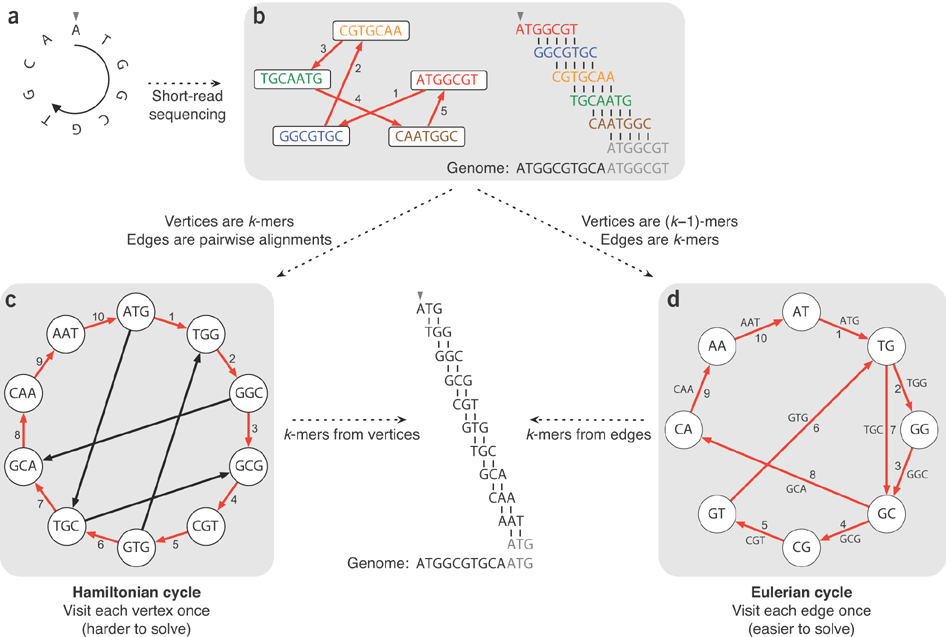
\includegraphics[width=\textwidth]{/home/nicholas/GitHub/FB/Ecoli_comparative_genomics/doc/presentations/MyNUIG(mnuigtheme)/frequentFigs/Compeau2011.png}\\\tiny {Source: Compeau2011}
\end{frame}


\begin{frame}[fragile]
  \frametitle{Problems}
  \centering
  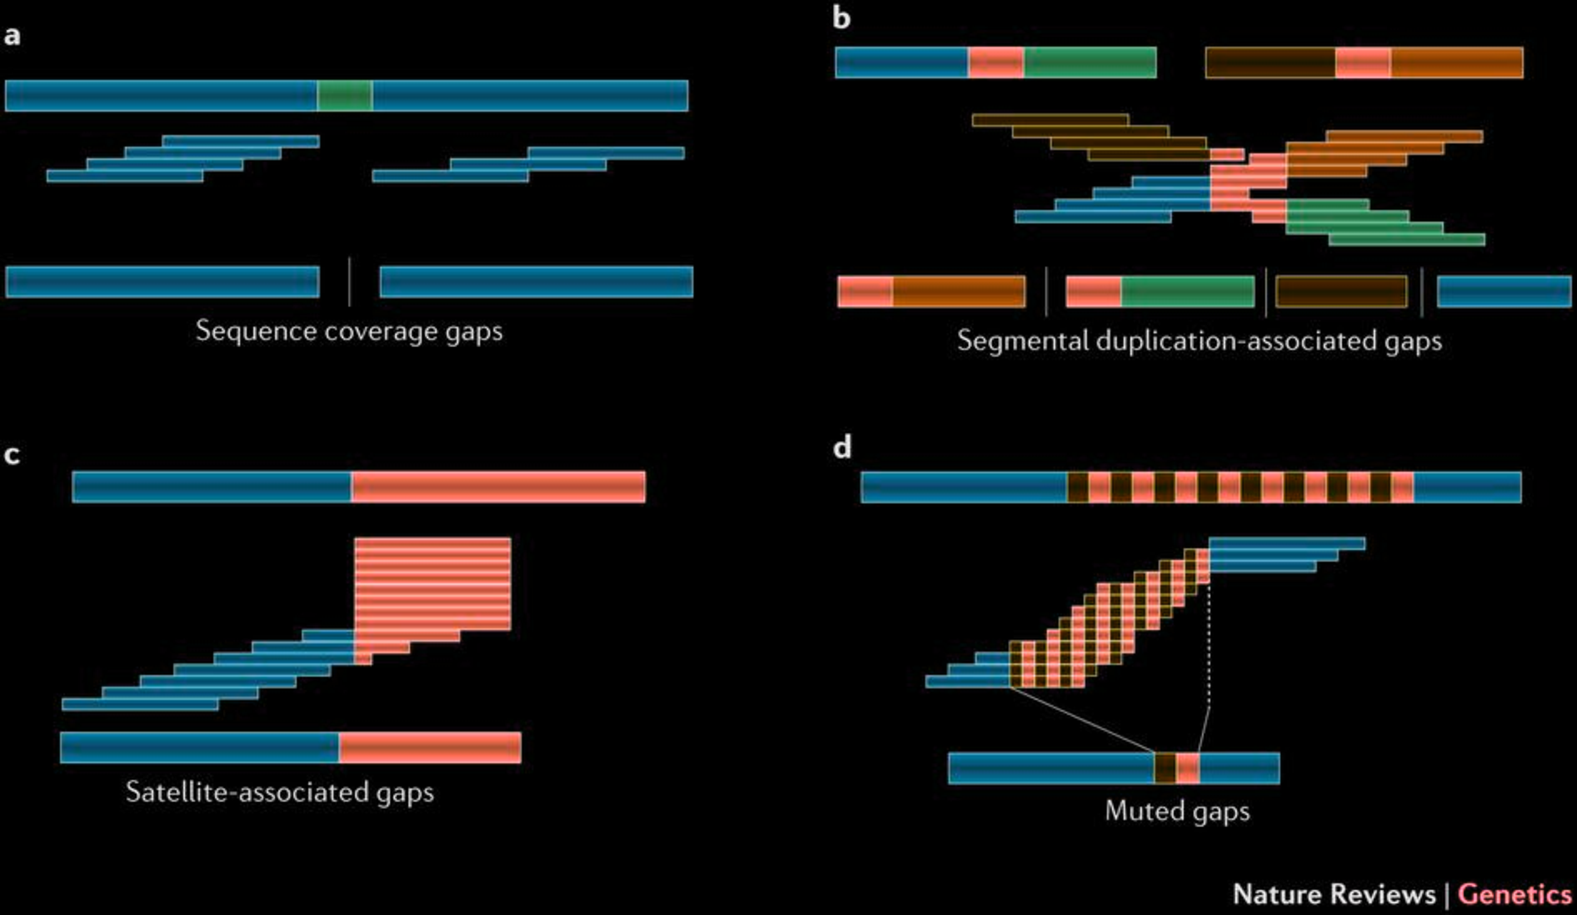
\includegraphics[width=.95\textwidth]{/home/nicholas/GitHub/FB/Ecoli_comparative_genomics/doc/presentations/MyNUIG(mnuigtheme)/20161206_dc_figs/nature_invert.pdf}\\\tiny {Source:Chaisson2015}
\end{frame}

% \begin{frame}[fragile]
%   \frametitle{Eulerian Paths with Repeats}
%   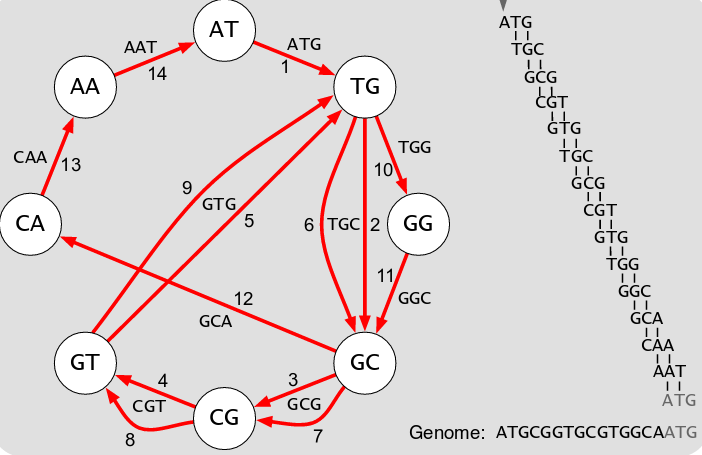
\includegraphics[width=\textwidth]{/home/nicholas/GitHub/FB/Ecoli_comparative_genomics/doc/presentations/MyNUIG(mnuigtheme)/frequentFigs/Compeau2_2011.png}\\\tiny {Source\cite{Compeau2011}}
% \end{frame}

% \begin{frame}[fragile]
%   \centering
%   
\includegraphics[width=.9\textwidth,trim=1cm .2cm 1cm .2cm, clip]{/home/nicholas/GitHub/FB/Ecoli_comparative_genomics/doc/presentations/MyNUIG(mnuigtheme)/frequentFigs/onedoesnot.jpg}\\\tiny {Source: T. Seemann}
% \end{frame}

\begin{frame}[fragile]
  \frametitle{Problem Regions}
  {\LARGE Repeated regions cannot be resolved with kmers shorter than the repeat!}
\only<1>{\vskip4.0cm}
\only<2>{\begin{figure}
\begin{tabular}{cccc}
  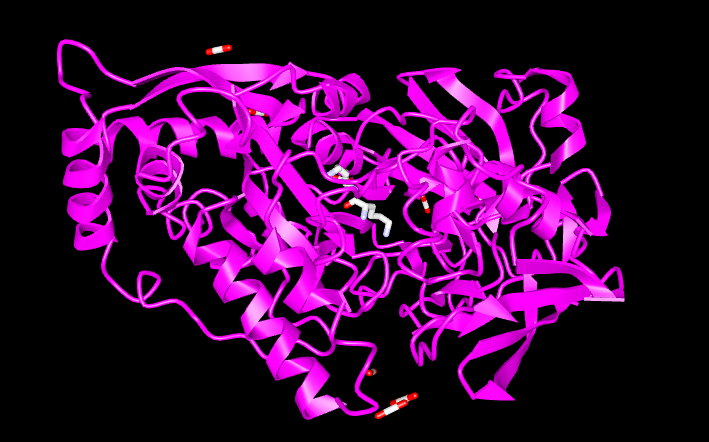
\includegraphics[width=.25\textwidth]{~/GitHub/FB/Ecoli_comparative_genomics/doc/presentations/MyNUIG(mnuigtheme)/frequentFigs/oppa.png} & 
\includegraphics[width=.15\textwidth]{~/GitHub/FB/Ecoli_comparative_genomics/doc/presentations/MyNUIG(mnuigtheme)/frequentFigs/plasmid_D.pdf} & 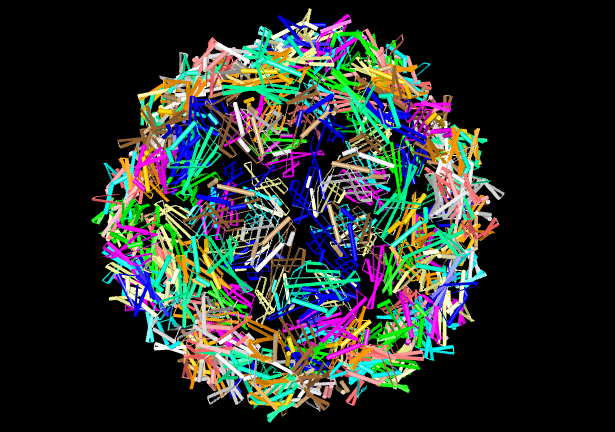
\includegraphics[width=.25\textwidth]{~/GitHub/FB/Ecoli_comparative_genomics/doc/presentations/MyNUIG(mnuigtheme)/frequentFigs/psuedo_prophage.png} & 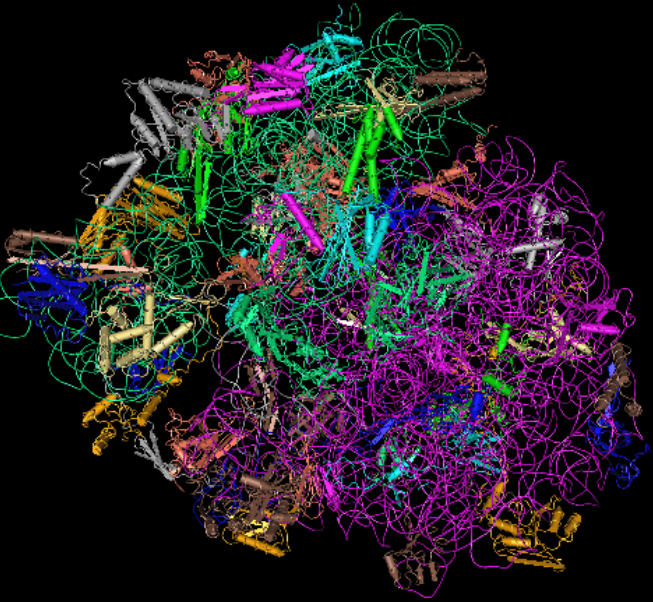
\includegraphics[width=.2\textwidth]{~/GitHub/FB/Ecoli_comparative_genomics/doc/presentations/MyNUIG(mnuigtheme)/frequentFigs/ribo.png} \\
 Transporters &  $\Omega$ Plasmids &  Prophages &  Ribosomes\\[6pt]
 % 
\includegraphics[width=.3\textwidth]{~/GitHub/FB/Ecoli_comparative_genomics/doc/presentations/MyNUIG(mnuigtheme)/frequentFigs/plasmid_D.pdf} &   
\includegraphics[width=.3\textwidth]{~/GitHub/FB/Ecoli_comparative_genomics/doc/presentations/MyNUIG(mnuigtheme)/frequentFigs/plasmid_D.pdf} & \\
 % (d) fourth & (e) fifth & \\[6pt]
\end{tabular}
\end{figure}}
\end{frame}

\section{Is it Hopeless?}
\begin{frame}
  \frametitle{Genome Finishing}
  \centering
  % \hspace*{-1cm}
  \begin{tabular}{l|l|l}
    \hline
    method & benefits & drawbacks\\
    \hline
    PCR + Sanger & it works & its difficult \\
    re-sequencing & improve coverage & issues with repeats \\
    long reads & solves repeats & cost, availability \\
    reference assisted & easy to perform & not reliable \\
    genome finishing tools & many options & many options \\
  \end{tabular}
\end{frame}

\begin{frame}
  \frametitle{Genome Finishing Tools}
  \centering
\begin{table}[]
\centering
% \caption{My caption}
\label{my-label}
\resizebox{\textwidth}{!}{
\begin{tabular}{lll}
  Tool                          & Reference                     & Method Summary                                                                                                                                                    \\
  \hline
  GapFiller    & {[}Boetzer2012{]}             & utilize paired end reads
                                                \\  GapCloser/IMAGE & {[}Luo2012{]}, {[}Tsai2010{]} & iteratively maps reads to contigs\\
                          CloG                          & {[}Yang2011{]}                & uses trimmed de novo contigs in hybrid assembly\\
                 FGap                          & {[}Piro2014,Guizelini2016{]}  & uses BLAST to find potential gap closures\\
        GFinisher                     & {[}Guizelini2016{]}           & uses GC-skew to refine assemblies\\                                         GapFiller    & {[}Nadalin2012{]}             &  uses a hash-based method to produce “long-reads”\\
                                                 CONTIGuator                   & {[}Galardini2011{]}           & generates a contig map and PCR primer sets to validate in the lab\\              \\
  Konnector                     & {[}Vandervalk2015{]}          & uses  a Bloom filter representation of a de Bruijn graph                                                         \\
\end{tabular}}
\end{table}
\end{frame}

\begin{frame}[fragile]
  \frametitle{Possible Solution}
  \begin{figure}
% see

\definecolor{cb3b3b3}{RGB}{179,179,179}
\definecolor{cffaaaa}{RGB}{255,170,170}
\definecolor{cdeaa87}{RGB}{222,170,135}
\definecolor{cff9955}{RGB}{255,153,85}


\begin{tikzpicture}[y=0.80pt, x=0.80pt, yscale=-1.00000, xscale=1.000000, inner sep=0pt, outer sep=0pt]
\path[draw=black,fill=cb3b3b3,miter limit=4.00,draw opacity=0.000,line
  width=0.137pt,rounded corners=0.0000cm] (98.0545,56.3976) rectangle
  (304.3740,66.3267);
\path[draw=black,fill=cffaaaa,miter limit=4.00,draw opacity=0.000,line
  width=0.061pt,rounded corners=0.0000cm] (92.8397,84.3501) rectangle
  (132.8746,94.3743);
\path[draw=black,fill=cffaaaa,miter limit=4.00,draw opacity=0.000,line
  width=0.061pt,rounded corners=0.0000cm] (152.8397,102.3501) rectangle
  (192.8746,112.3743);
\path[draw=black,fill=cffaaaa,miter limit=4.00,draw opacity=0.000,line
  width=0.061pt,rounded corners=0.0000cm] (102.8397,102.3501) rectangle
  (142.8746,112.3743);
\path[draw=black,fill=cffaaaa,miter limit=4.00,draw opacity=0.000,line
  width=0.061pt,rounded corners=0.0000cm] (122.8397,122.3501) rectangle
  (162.8746,132.3743);
\path[draw=black,fill=cffaaaa,miter limit=4.00,draw opacity=0.000,line
  width=0.061pt,rounded corners=0.0000cm] (139.2682,84.4929) rectangle
  (179.3032,94.5172);
\path[draw=black,fill=cffaaaa,miter limit=4.00,draw opacity=0.000,line
  width=0.061pt,rounded corners=0.0000cm] (228.5539,87.3501) rectangle
  (268.5889,97.3743);
\path[draw=black,fill=cffaaaa,miter limit=4.00,draw opacity=0.000,line
  width=0.061pt,rounded corners=0.0000cm] (246.8397,106.3501) rectangle
  (286.8746,116.3743);
\path[draw=black,fill=cffaaaa,miter limit=4.00,draw opacity=0.000,line
  width=0.061pt,rounded corners=0.0000cm] (272.8397,122.3501) rectangle
  (312.8746,132.3743);
\path[draw=black,fill=cffaaaa,miter limit=4.00,draw opacity=0.000,line
  width=0.061pt,rounded corners=0.0000cm] (262.8397,142.3501) rectangle
  (302.8746,152.3743);
\path[draw=black,fill=cffaaaa,miter limit=4.00,draw opacity=0.000,line
  width=0.061pt,rounded corners=0.0000cm] (226.8397,124.3501) rectangle
  (266.8746,134.3743);
\path[draw=black,fill=cdeaa87,miter limit=4.00,draw opacity=0.000,line
  width=0.061pt,rounded corners=0.0000cm] (187.8397,145.9215) rectangle
  (227.8746,155.9457);
\path[draw=black,fill=cffaaaa,miter limit=4.00,draw opacity=0.000,line
  width=0.061pt,rounded corners=0.0000cm] (252.8397,72.3501) rectangle
  (292.8746,82.3743);
\path[draw=black,fill=cff9955,miter limit=4.00,draw opacity=0.000,line
  width=0.069pt,rounded corners=0.0000cm] (182.8517,32.3551) rectangle
  (234.2911,42.3693);

\end{tikzpicture}

\caption{Bridge Reconstruction. Pink fragments are reads.  Grey shows the gene of interest with interupted coverage. Orange fragemnt is a pseudoread generated from this situation under the hypothesis that the beige fragment exists but is underrepresented}
\label{fig:bridge_rec}
\end{figure}
\end{frame}


% \begin{frame}[fragile]
%   \frametitle{Problem Regions}
%   \begin{itemize}
%     \item Transport proteins
%     \item Phage
%     \item Integrated plasmids
%     \item {\Large\textbf rRNAs}
%     \end{itemize}
% \end{frame}
\begin{frame}[fragile]
  \frametitle{Problem Regions}
  {\LARGE Repeated regions cannot be resolved with kmers shorter than the repeat!}
  \begin{figure}
\begin{tabular}{cccc}
  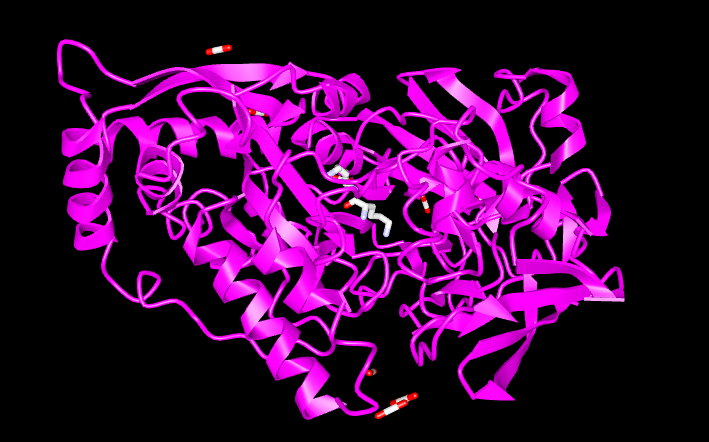
\includegraphics[width=.25\textwidth]{~/GitHub/FB/Ecoli_comparative_genomics/doc/presentations/MyNUIG(mnuigtheme)/frequentFigs/oppa.png} & 
\includegraphics[width=.15\textwidth]{~/GitHub/FB/Ecoli_comparative_genomics/doc/presentations/MyNUIG(mnuigtheme)/frequentFigs/plasmid_D.pdf} & 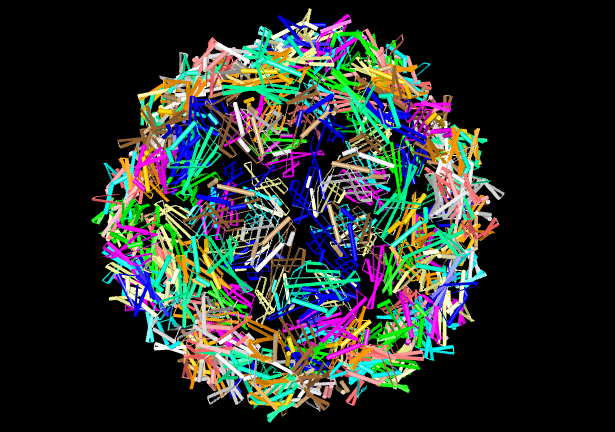
\includegraphics[width=.25\textwidth]{~/GitHub/FB/Ecoli_comparative_genomics/doc/presentations/MyNUIG(mnuigtheme)/frequentFigs/psuedo_prophage.png} & 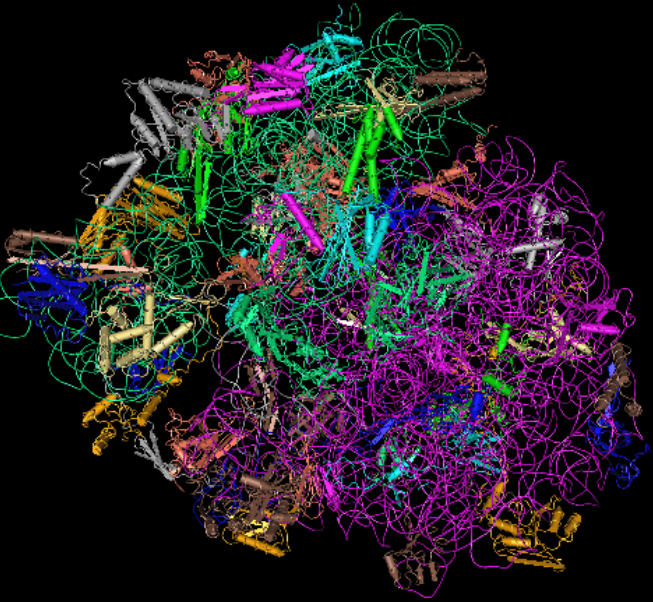
\includegraphics[width=.2\textwidth]{~/GitHub/FB/Ecoli_comparative_genomics/doc/presentations/MyNUIG(mnuigtheme)/frequentFigs/ribo.png} \\
  Transporters &  $\Omega$ Plasmids &  Prophages &  \alert<2>{Ribosomes}\\[6pt]
 % 
\includegraphics[width=.3\textwidth]{~/GitHub/FB/Ecoli_comparative_genomics/doc/presentations/MyNUIG(mnuigtheme)/frequentFigs/plasmid_D.pdf} &   
\includegraphics[width=.3\textwidth]{~/GitHub/FB/Ecoli_comparative_genomics/doc/presentations/MyNUIG(mnuigtheme)/frequentFigs/plasmid_D.pdf} & \\
 % (d) fourth & (e) fifth & \\[6pt]
\end{tabular}
\end{figure}
\end{frame}

\begin{frame}[fragile]
  \frametitle{rDNA}
  rDNA: ribosomal DNA operon
  \begin{itemize}
    \item Prokaryotes: 16S, 23S, 5S
    \item Conserved within taxa
    \item Repeated within the genome (1x to >14x)
    \end{itemize}
\end{frame}

\begin{frame}[fragile]
\frametitle{Hypotheses}
  \begin{enumerate}
  \item Since the rDNA structure is conserved within taxa, rDNA flanking regions may be conserved
  \item Regions flanking the rDNA region will be unique within genomes
  \item If flanking regions are unique, they can be used to build ``long reads''
\end{enumerate}
\end{frame}

\section{Hypothesis 1: ribosomal Operons}

\begin{frame}[fragile]
  \frametitle{rDNA flanking regions are conserved conserved}
  \centering
  \includegraphics[width=.49\textwidth]{~/GitHub/FB/Ecoli_comparative_genomics/doc/notebook/figures/screengrab_comp16s1.png}
  \hfill
  \includegraphics[width=.49\textwidth, trim=0 2mm 0 0, clip]{~/GitHub/FB/Ecoli_comparative_genomics/doc/notebook/figures/screengrab_comp16s2.png}
\end{frame}
\begin{frame}[fragile]
  \frametitle{rDNA flanking regions are conserved}
  \hspace*{1cm}
  \includegraphics[width=.8\textwidth]{~/GitHub/FB/Ecoli_comparative_genomics/doc/notebook/figures/screengrab_comp16s3.png}
\end{frame}

\section{Hypothesis 2: Flanking Uniqueness}

\begin{frame}[fragile]
  \frametitle{Flanking regions are unique within genome}
  \hspace*{-1cm}
  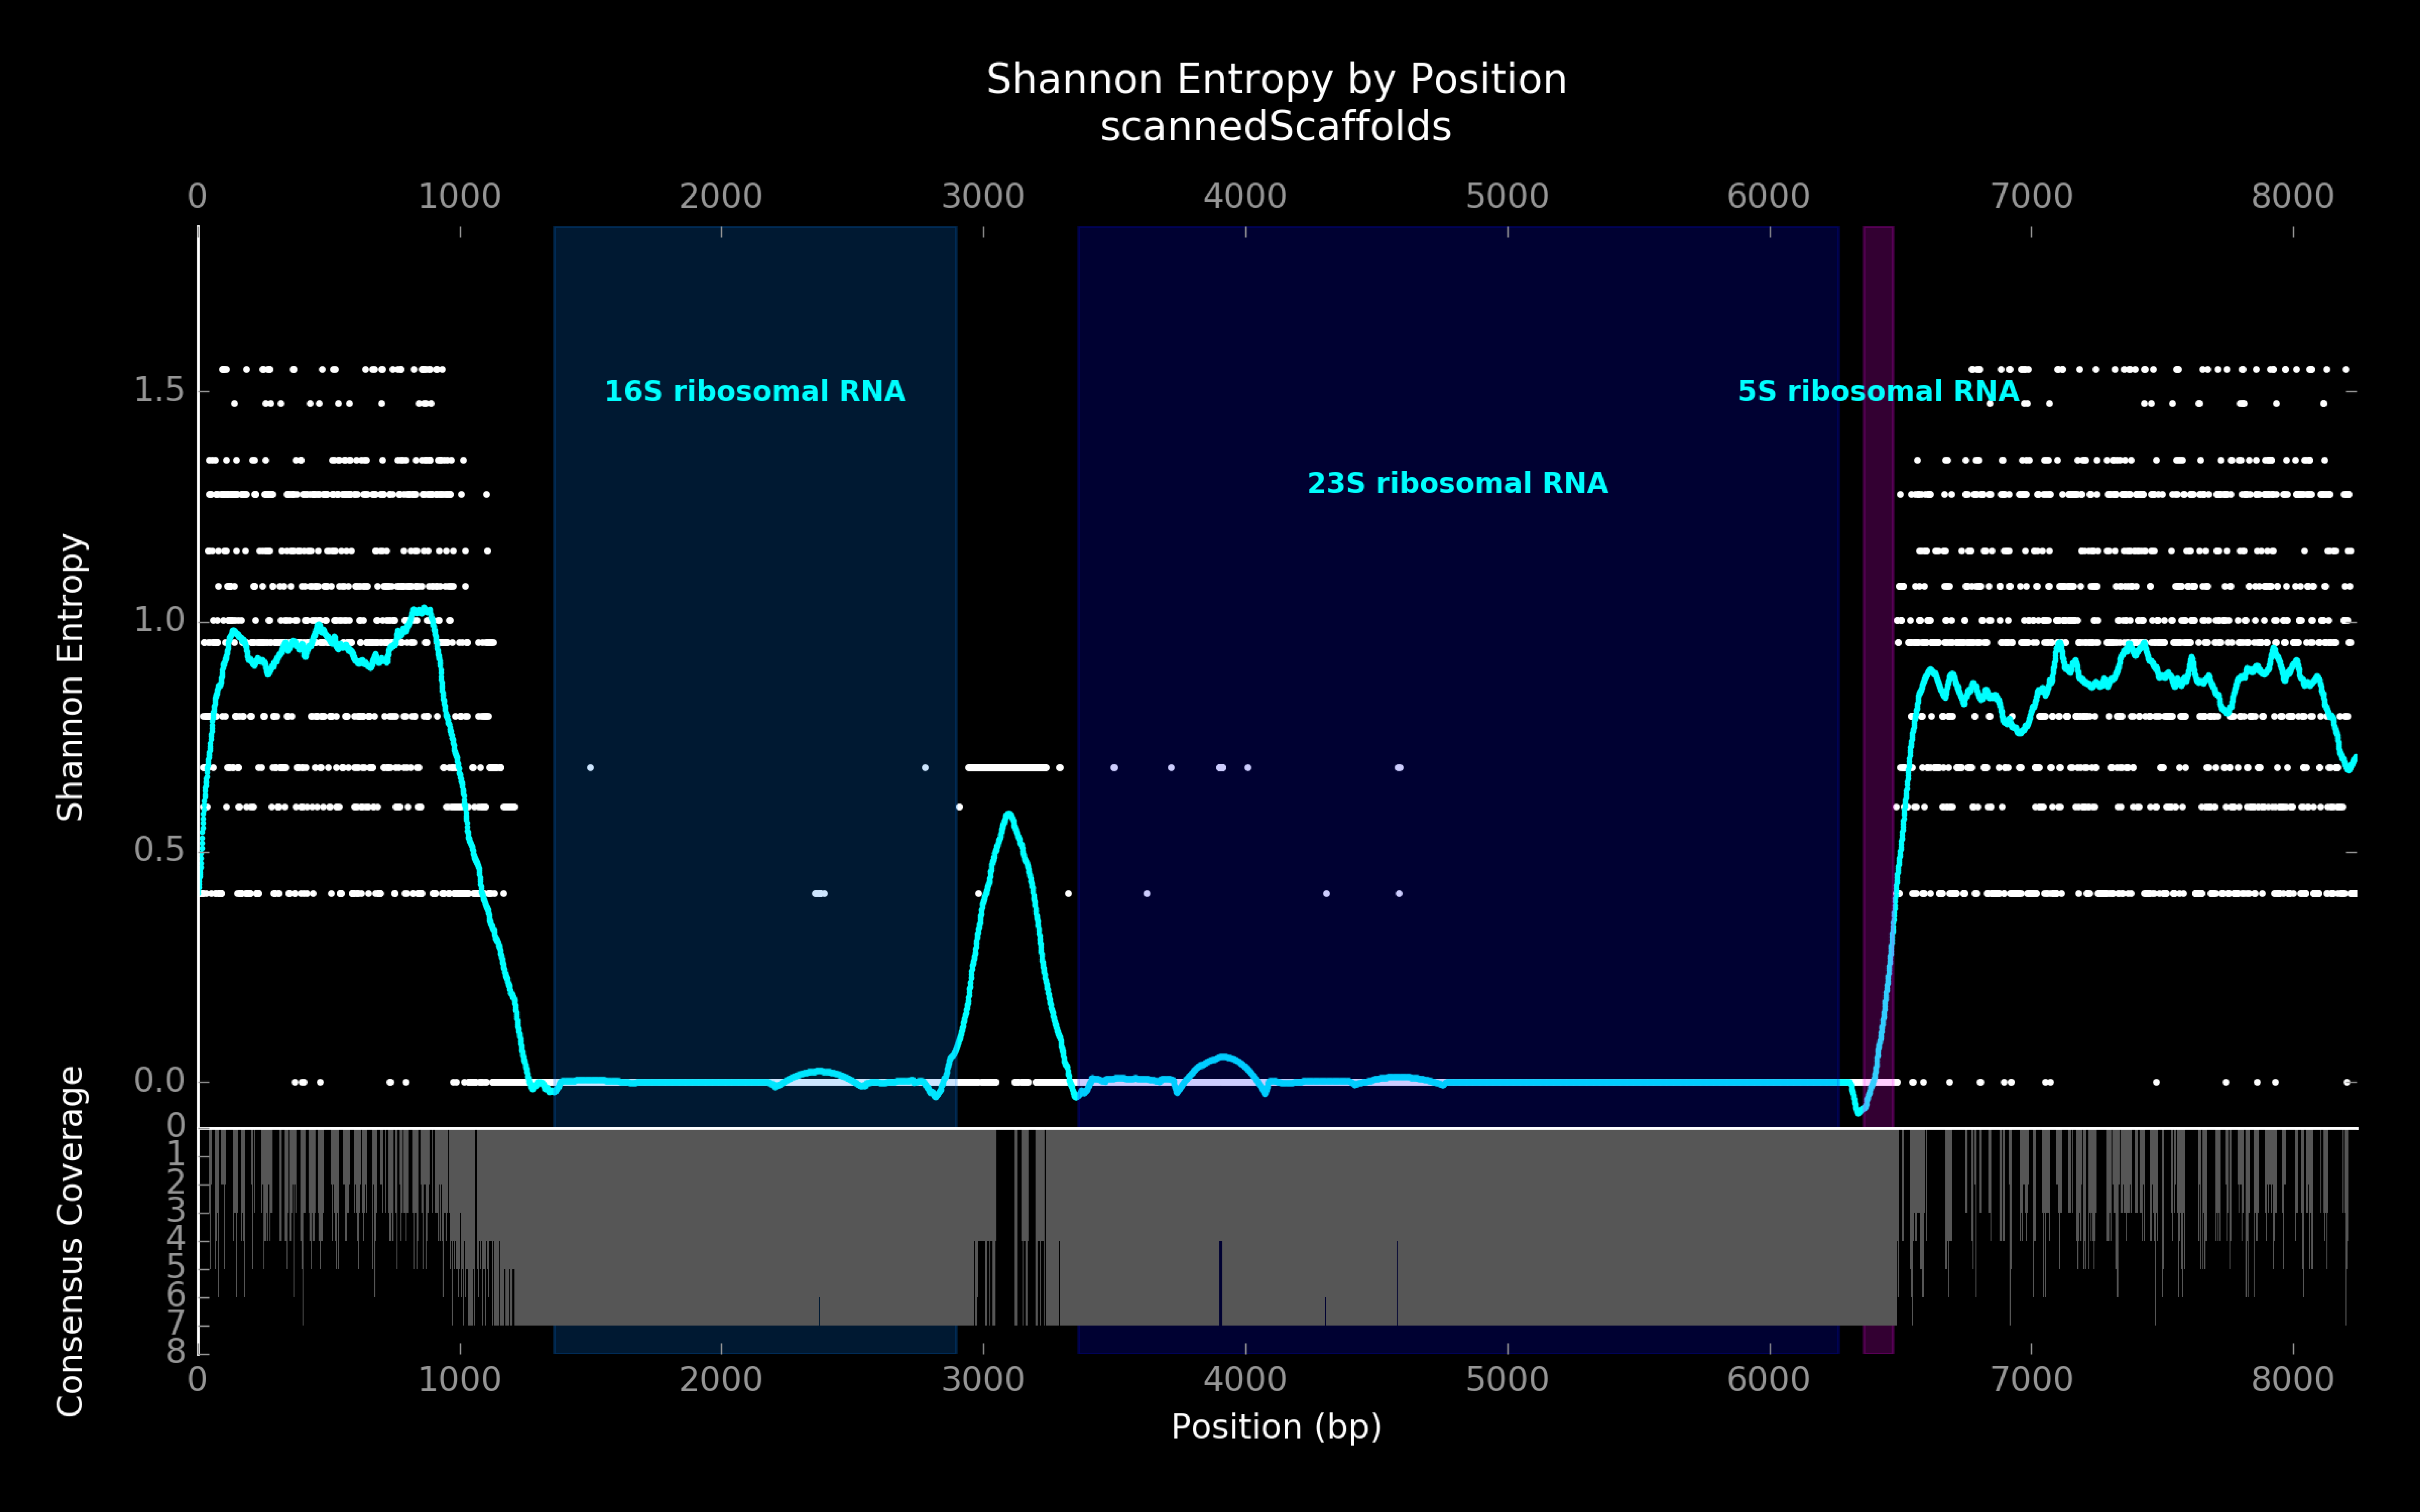
\includegraphics[width=\paperwidth]{~/GitHub/FB/Ecoli_comparative_genomics/doc/presentations/MyNUIG(mnuigtheme)/frequentFigs/entropy_coli_D.png}
\end{frame}


\section{Hypothesis 3: Long Read Construction}

% \begin{frame}[fragile]
%   \frametitle{Can flanking regions be used to improve assembly?}

% \end{frame}
\begin{frame}[fragile]
  \frametitle{riboSeed}
    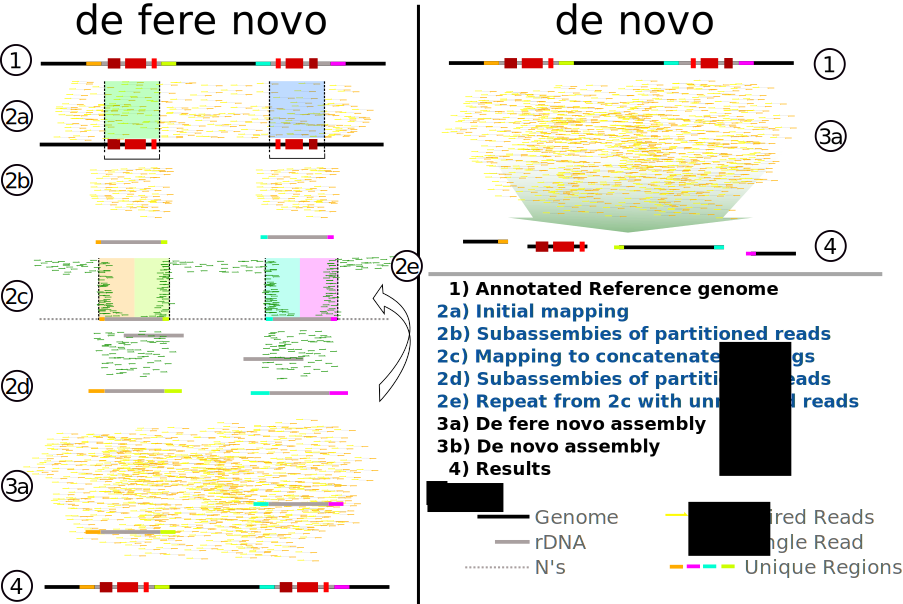
\includegraphics[width=\textwidth]{../../notebook/figures/riboSeed/riboSeed_v8.png}\\

\end{frame}


\begin{frame}[fragile]
  \frametitle{riboSeed}
  % riboSeed:
  \begin{itemize}
  \item Automated method for constructing select ``long reads'' from Illumina data
  \item Written in python3 and R, wrapping barrnap, SMALT, SPAdes, and samtools
  \item 5 stages:
  \begin{enumerate}
    \item Identify rDNA clusters
    \item Extracts reads mapping to a cluster
    \item Assemble into long reads
    \item Repeat (3x default) to extend
    \item Submit rDNA long reads to de novo assembly

  \end{enumerate}
  \end{itemize}

\end{frame}

\begin{frame}[fragile]
  \frametitle{riboSeed v0.3.06}
  % riboSeed:
  \begin{itemize}
  \item Adjusts ``trustworthiness'' of long reads based on mapping
  \item Deals with rDNAs near origin
  \item Includes depth-of-coverage tool
  \end{itemize}

\end{frame}

\section{Does it work?}

\begin{frame}[fragile]
  \frametitle{Benchmarking}
  \begin{enumerate}
  \item synthetic reads on synthetic genome (7 \textit{E. coli Sakai} rDNAs separated by 6kb random sequence)
  \item synthetic reads on real genome
  \item short reads from hybrid assembly
  \item GAGE-B datasets
  \end{enumerate}

\end{frame}

\begin{frame}[fragile]
  \frametitle{Synthetic reads on synthetic genome}
  \hspace*{-0cm}
  \includegraphics[width=\textwidth]{/home/nicholas/GitHub/FB/Ecoli_comparative_genomics/doc/notebook/figures/20161005_toy_data.png}
\end{frame}

\begin{frame}[fragile]
  \frametitle{Synthetic reads on real genome}
  \hspace*{-0cm}
  \includegraphics[width=\textwidth]{/home/nicholas/GitHub/FB/Ecoli_comparative_genomics/doc/notebook/figures/20160919_mauve.png}
\end{frame}

\begin{frame}[fragile]
  \frametitle{Benchmarking with hybrid assembly}
  \begin{itemize}
  \item Successfull assembly across all 4 rDNAs
  \item Highly accurate reconstruction (3 SNPs per 8000bp)
  \end{itemize}
\end{frame}

\section{Challenges}
\begin{frame}[fragile]
  \frametitle{Reference Reliability}
  \hspace*{-0cm}
  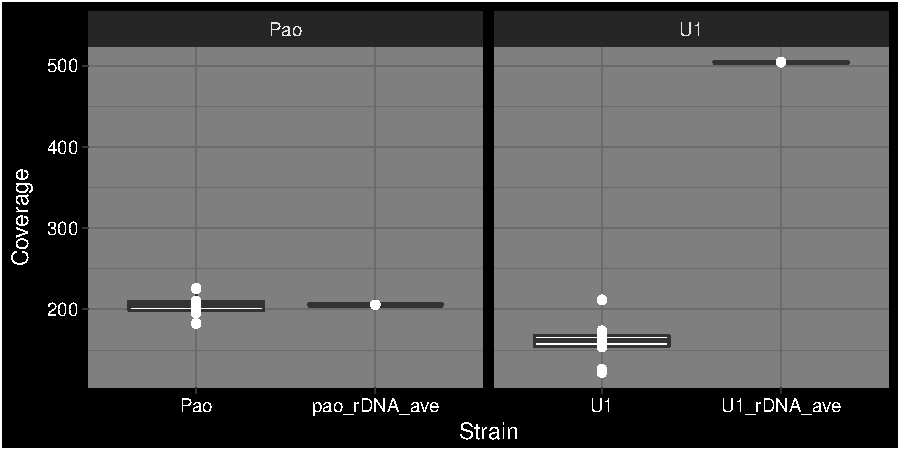
\includegraphics[width=\textwidth]{/home/nicholas/GitHub/FB/Ecoli_comparative_genomics/doc/presentations/MyNUIG(mnuigtheme)/frequentFigs/dumb_box.pdf}
\end{frame}

\begin{frame}[fragile]
  \frametitle{Other Challenges}
\begin{itemize}
\item Data Availability
\item Cross Platform Performance
\item Recruiting Beta Testing
\end{itemize}
\end{frame}




\section{Conclusions}
 \begin{frame}[fragile]
  \frametitle{Potential Downsides}
\begin{enumerate}
  \item Unpredictable
  \item Single problem/solution
  \item Biased by reference
\end{enumerate}
\end{frame}

 \begin{frame}[fragile]
  \frametitle{Summary}
  \begin{itemize}[<+- | alert@+>]
  \item The architecture of bacterial genomes can aid assembly
  \item rDNA flanking regions are unique within a genome
  \item riboSeed improves assemblies at best
  \item riboSeed doesn't work on in all cases, but rarely introduces errors
  \end{itemize}
\end{frame}

\begin{frame}[fragile]
  \frametitle{Next Steps}
  \begin{itemize}
  \item Benchmark against GAGE-B
  \item Benchmark against more hybrid assembly studies
  \item Find early indicator
  \item Apply to fungal genomic
  \item Apply to other conserved regions
  \end{itemize}
\end{frame}



\begin{frame}
%\addbibresource{myreferences.bib}
\bibliography{/home/nicholas/GitHub/FB/library}
\end{frame}

\setbeamertemplate{itemize items}[square]
\begin{frame}{Acknowledgments}
  \begin{columns}[onlytextwidth]
    \column{0.5\textwidth}
    \includegraphics[height=1cm]{../stock_logos/NUI_Galway_BrandMark_A_K.eps}\\
      \begin{itemize}
        \item \textbf{Fiona Brennan}
        \item \textbf{Florence Abram}
        \item Matthias Waibel
        \item Camilla Thorn
        \item Stephen Nolan
        \end{itemize}
        \vfill
      % NUIG Maths
      % \begin{itemize}
      %   \item Pilib O'Bryan
      % \end{itemize}

    \column{0.5\textwidth}
    
\includegraphics[height=1.1cm]{~/GitHub/FB/Ecoli_comparative_genomics/doc/presentations/MyNUIG(mnuigtheme)/frequentFigs/jhi_dark.png}\\
      \begin{itemize}
      \item \textbf{Leighton Pritchard}
        \item \textbf{Ashleigh Holmnes}
        \end{itemize}
        \vskip 1.2cm
        \only<1>{\vskip .55cm}
        \alert<2>{\only<2>{\LARGE \textbf{Questions?}}}
  \end{columns}
\end{frame}



% \plain{}{Questions?}

\end{document}
